\subsubsection{TDC testing}

{\it Important figures:\\
integral nonlinearity (INL) -- cable delay plots \\
differential nonlinearity (DNL) -- white histogram, channel width distribution\\
intrinsic time resolution\\
dithering mode on versus off\\
}



The properties of the TDC determine the most basic unit of time resolution. Resolution, differential nonlinearity (DNL), and integral nonlinearity (INL), were measured for common-start CAMAC modules (Phillips Scientific PS7186 and Caen C414) and a newer pipeline VME module (Caen V1290N). Neither CAMAC module met the manufacturer's specifications, but the Caen VME module V1290N performed acceptably, which was one factor in the choice to use VME during our prototype development.  Ultimately, however, the pipeline class of TDC is required for a more basic reason: it allows for the decoupling of the coincidence trigger from the timing trigger, which removes all electronic logic system contributions other than the discriminator from the time resolution.

In order to determine the DNL profile of each module, a random start signal and periodic stop signal are fed to the TDC. The stop signal arrives at the TDC in any fixed-width time interval with equal probability.  Thus, after a large number of events, a uniform distribution of counts per time interval (bin) is expected in the ideal case. Deviations from the ideal result minus statistical noise reflect the TDC's DNL.

\begin{figure}[]
\centering
\includegraphics[width=0.8\textwidth]{evan/fig_evan_tdc_testing/placeholder.eps} %{cDNL.pdf}
\caption{The DNL histogram (left) deviates from an ideal uniform distribution, indicated by the dotted line, with a standard deviation of 92 counts (right), so the relative nonlinearity is $\frac{92}{3635} = 2.5\%$. After compensating for the statistical contribution of $\frac{\sqrt{3635}}{3635} = 1.66\%$, the relative DNL is $1.9\%$. The sloped edges result from the $25\:ns$ variability in the V1290N's timing window with respect to the trigger. The periodic needles, again at $25\:ns$ intervals, result from INL compensation on the TDC chip level.\cite{v1290n-man} The additional interference at TDC value $0$ results from crosstalk between the two signals.\label{fig:tdcDNL}}
\end{figure}

A radioactive source of Sr-90, placed on a counter, provides the random signals, which are converted to NIM logic signals by a leading edge discriminator (Phillips Scientific 705) for timing. In parallel, a timing unit (Phillips Scientific 794) provides logic pulses with a period greater than the TDC full range for the common-start CAMAC TDCs and a period of $200\:ns$ for the pipeline VME TDC. The random signal serves as the reference signal, and the periodic signal, sent to all channels via a logic fan in/out (LeCroy 429A), serves as the channel-specific stop. A TDC value distribution and its corresponding bin-width distribution are histogrammed in Fig.$\:$\ref{fig:tdcDNL}, and for comparison, the DNL histograms of PS7186 and C414 are illustrated in Fig.$\:$\ref{fig:tdcDNLcamac}.

\begin{figure}[]
\centering
\includegraphics[width=0.8\textwidth]{evan/fig_evan_tdc_testing/placeholder.eps} %{dnl_camac.pdf}
\caption{DNL histograms for the Phillips Scientific 7186 (left) and the Caen 414 (right), compared with that of the Caen V1290N (Fig.$\:$\ref{fig:tdcDNL}, left), illustrate different nonlinearity signatures. The PS7186 and C414 are 12-bit CAMAC modules with limited ranges. The entire $100\:ns$ range (12-bit) is usable in the PS7186, but the high nonlinearity below bin 1100 of the C414 restricts the usable range to only about $60\:ns$.\label{fig:tdcDNLcamac}}
\end{figure}

\begin{figure}[]
\centering
\includegraphics[width=0.8\textwidth, height=2.5in]{evan/fig_evan_tdc_testing/placeholder.eps} %{tdc_c414_cableDelays.pdf}
\includegraphics[width=0.8\textwidth, height=2.5in]{evan/fig_evan_tdc_testing/placeholder.eps} %{tdc_cal.pdf}
\caption{Typical TDC calibration results illustrated for the Caen C414. Two copies of the same signal are used as start and stop times, with the latter being delayed with measured cable lengths in $5\:ns$ increments (top). The typical peak width corresponds to $\sigma=0.7\:bins$. The mean TDC value of each peak is plotted with its corresponding measured delay (bottom) to get the TDC sensitivity and offset (parameters $p1$ and $p0$, respectively).\label{fig:tdcDelays}}
\end{figure}

Calibration of the TDCs was accomplished by applying variable, oscilloscope-measured cable delays in $5\:ns$ increments. Figure$\:$\ref{fig:tdcDelays} demonstrates the calibration procedure where, in the illustrated case of the Caen C414, the average bin width is $25.11\:ps$ with an offset of $2.8\:ns$. Each $5ns$-interval peak includes 1000 entries and has a width corresponding to $0.6\:\textrm{bins}<\sigma<0.8\:\textrm{bins}$. Results for each TDC are tabulated in Table$\:$\ref{tab:TDC}.

\begin{table}[]
\centering
\caption{TDC Summary.}
\begin{tabular}{c r r r r r r }
\hline
Model & DNL$_{\sigma}$ & DNL$_{max}$ & Range(ns) & Offset(ns) & Bin Size(ps) & Resolution(ps) \\
\hline\hline
PS7186 & 9.8\% & 48.9\% & 100 & 18-21 & 24.98 & 19.0 \\
C414 & 8.9\% & 135.6\% & 72 & 0-5 & 25.11 & 17.5 \\
V1290N & 1.9\% & 41.1\% & N/A & N/A & 24.75 & 32.5 \\
\hline
\end{tabular}
\label{tab:TDC}
\end{table}

